%%%%%%%%%%%%%%%%%%%%%%%%%%%%%%%%%%%%%%%%%%%%%%%%%%%%%%%%%%%%%%%%%
% Qualificacao de Doutorado / Dept Fisica, CFM, UFSC            %
% Eduardo@UFSC - 2015                                           %
%%%%%%%%%%%%%%%%%%%%%%%%%%%%%%%%%%%%%%%%%%%%%%%%%%%%%%%%%%%%%%%%%

%:::::::::::::::::::::::::::::::::::::::::::::::::::::::::::::::%
%                                                               %
%                          Capítulo 3                           %
%                                                               %
%:::::::::::::::::::::::::::::::::::::::::::::::::::::::::::::::%

%***************************************************************%
%                                                               %
%                           Amostra                             %
%                                                               %
%***************************************************************%

\chapter{Amostra de galáxias}
\label{sec:amostra}

Nem todas as regiões das galáxias que estudamos têm medidas das linhas espectrais necessárias para
este estudo. Essa falta não é um defeito de observação e sim uma característica intrínseca de
determinada região. As linhas em emissão geralmente estão ligadas ao gás e nem todas as partes da
galáxia possuem gás. Nesse capítulo vamos descrever todas as características e máscaras impostas em
nossa amostra. Faremos um breve comentário sobre a classificação morfológica destas galáxias, além
de calcular e exemplificar os perfis radiais que utilizaremos em nossas discussões futuras.

\section{Artigo - CALIFA, the Calar Alto Legacy Field Area survey III. Second public data
release.}

Esse artigo (Apêndice \ref{apendice:GBetal2015a}) descreve uma amostra de 200 galáxias que tiveram
seus dados liberados no segundo {\em data release} do CALIFA (DR2) passando por todas as
configurações de observação, procedimentos de redução dos dados, avaliação de erros e controle de
qualidade. Nosso grupo de populações estelares se encarregou de escrever alguns programas de análise
e gerar as imagens nas quais nos embasamos para avaliar a qualidade da síntese de populações
estelares com o \starlight em 170670 espectros para distintas posições em cada galáxia, além de
realizarmos uma comparação com os resultados para a amostra do DR1 \citep{Husemann.etal.2013a}.
Durante esse trabalho notamos que os resíduos reduziram sensivelmente desde a última versão. Esta
mesma análise nos ajudou a melhorar a máscara de remoção de linhas telúricas\footnote{Linhas
provenientes de fenômenos que ocorrem na Terra.} dos espectros. Também verificamos que os erros
relacionados aos espectros observados possuem uma distribuição muito próxima a uma gaussiana. Todas
os dados presentes nesse trabalho receberam o mesmo pré-processamento detalhado neste artigo.

\section{Definição da amostra deste trabalho}
\label{sec:amostra:definicao}

A amostra de galáxias deste trabalho faz parte da amostra total de galáxias do CALIFA. Os dados
passaram pelos mesmos pré-processamento e controle de qualidade daqueles liberados pelo DR2, porém
possui dados que ainda não foram disponibilizados publicamente, abarcando 226176 regiões (zonas) de
305 galáxias espirais. Cada uma dessas zonas dessa é composta por um ou mais pixels, com um espectro
resultante da soma dos espectros destes, para que tenhamos relação sinal-ruído maior ou igual a 20
na janela de normalização deste espectro. Esse procedimento, conhecido como {\em Voronoi binning},
está detalhado, juntamente com o procedimento de derivação das propriedades estelares através do
código \starlight para cada uma das regiões destas galáxias, em \citet{CidFernandes.etal.2013a}.

\subsection{Mascarando elementos e removendo {\em outliers}}
\label{sec:amostra:mask}

Para que possamos focar nossos estudos nas regiões de formação estelar, aplicamos uma máscara nos
dados selecionando as regiões que possuam:
\begin{itemize}
  \setlength\itemsep{0.2cm}
  \item medidas do fluxo integrado das linhas de \Hbeta, \oIII, \Halpha e \nII com relação
sinal-ruído maior do que 3;
  \item medidas para as seis propriedades comparadas neste capítulo:
  \begin{itemize}
    \item coeficiente de extinção proveniente da síntese - $\tauVS$;
    \item coeficiente de extinção estimado através do decremento de Balmer - $\tauVN$;
    \item densidade superficial da taxa de formação estelar calculado através da síntese -
$\SigmaSFR$;
	\item densidade superficial da taxa de formação estelar calculado através da luminosidade de
\Halpha - $\SigmaSFRN$;
	\item metalicidade média das populações estelares, pesada pela massa estelar - $\meanM{\log
Z_\star}$;
	\item metalicidade nebular - $\log(O/H)$.
  \end{itemize}
  \item fração de luz proveniente de populações estelares jovens maior que 0.05 (5\%) ($x_Y >
0.05$);
  \item $\tauV$ e $\tauVN$ maiores que 0.05;
  \item mais do que cinco zonas contribuindo para o cálculo dos perfis radiais;
  \item distância ao núcleo maior que 70\% do raio que contém metade da luz ({\em half-light radius}
  - HLR).
\end{itemize}
\noindent O que aqui chamamos de população jovem discutiremos um pouco mais adiante, na Sec.
\ref{sec:synvsneb:SFR}. A última imposição é feita para que não haja contaminação por zonas
do bojo da galáxia (partes centrais onde as linhas são produzidas por diferentes fenômenos físicos,
relacionados a um núcleo ativo). Esse valor (0.7 HLR) foi definido por nossos colaboradores
analisando as curvas de brilho das galáxias e representa um valor máximo para localização de zonas
centrais. 

Na Fig.\ \ref{fig:histosample} podemos ver os histogramas normalizados (a integral dentro do
intervalo do histograma é 1) de algumas propriedades de modo que evidencie os efeitos da máscara
que forma nossa amostra. Em vermelho temos as 226176 regiões em 305 galáxias e, em azul, as 16479
zonas de 184 galáxias (19 Sa, 38 Sb, 59 Sbc, 55 Sc e 13 Sd). É notável que nossa seleção busca zonas
mais densas e mais jovens (maior fração de populações jovens diminuindo a idade média). O corte mais
brusco em nossa amostra é devido a baixa relação sinal-ruído da linha de \oIII ($(S/N)_{\oIII} < 3$)
em 91142 zonas.
\begin{figure}
	\centering
	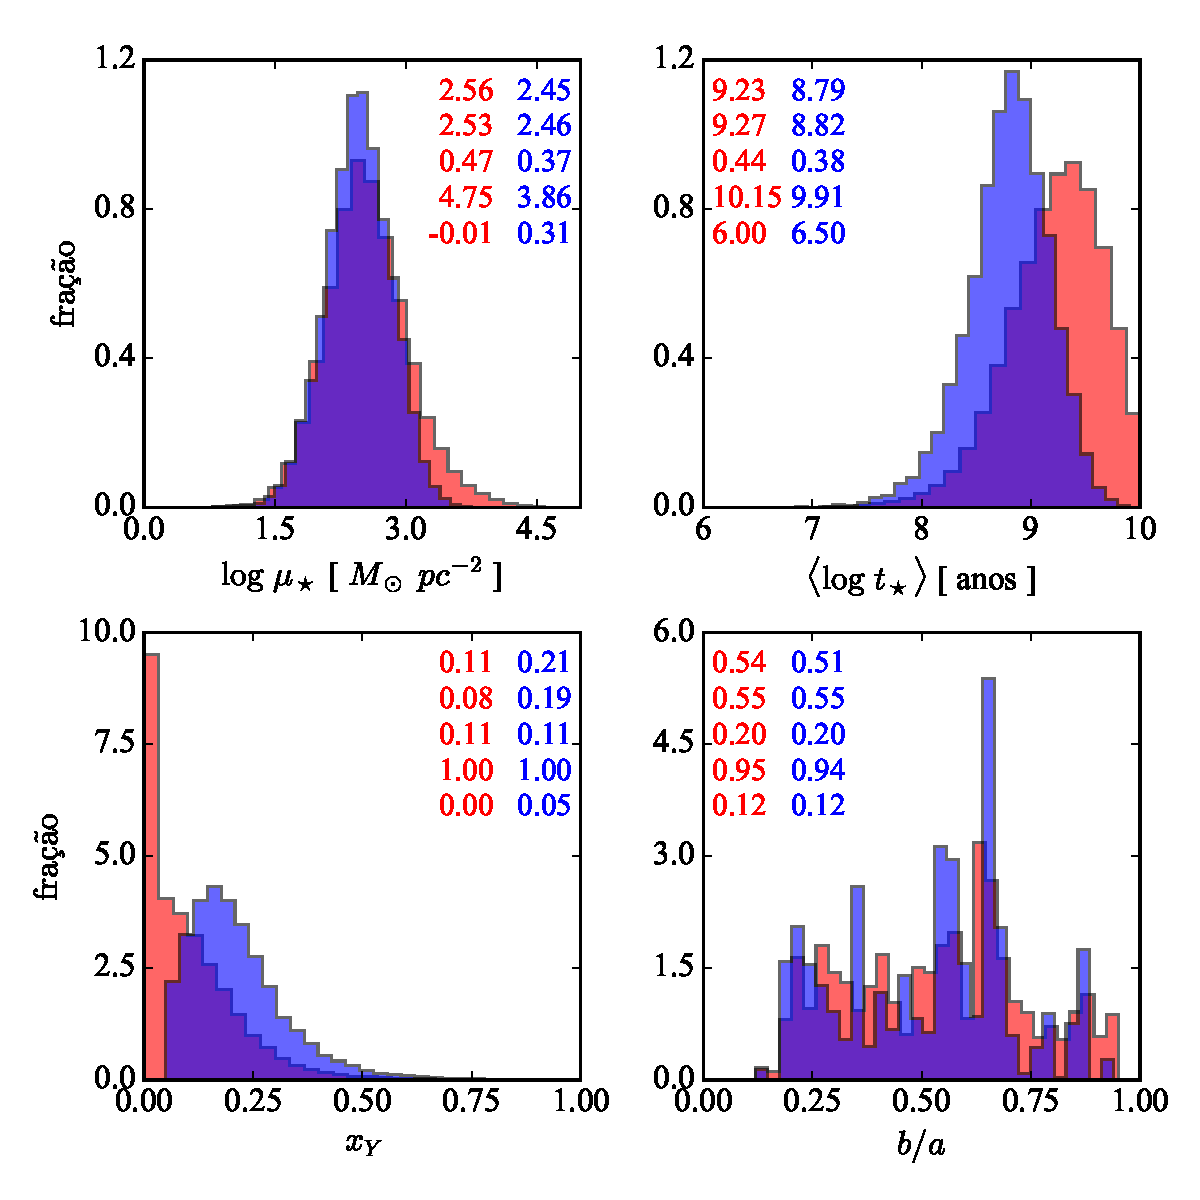
\includegraphics[width=0.99\textwidth]{figuras/histosample.pdf}
	\caption[Histogramas: densidade superficial de massa, idade média, fração de populações jovens e
	relação axial.] 
	{Histogramas da densidade superficial de massa ({\em painel a}), idade média das populações
estelares ({\em painel b}), fração de populações jovens ({\em painel c}) e relação axial ({\em
painel d}). Em vermelho temos a distribuição de valores de 226176 regiões em 305 galáxias e, em
azul, a de 16525 zonas de 184 galáxias resultantes da seleção. Em cada gráfico temos os valores da
média, mediana, desvio padrão, máximo e mínimo de cada distribuição.}
	\label{fig:histosample}
\end{figure}

\subsection{Classificação Morfológica}
\label{sec:amostra:morf}

Com tipos morfológicos variando entre Sa e Sd, massas estelares entre $10^9$ e $10^{11.5}\ M_\odot$
e populações estelares com idades médias entre $10^8$ e $10^{10}$ anos, podemos ver na Fig.
\ref{fig:amostraMorf} que as galáxias se ordenam de forma interessante quando agrupadas por tipo
morfológico, anticorrelacionando com a idade média estelar e a massa estelar ($M_\star$ e $t_\star$)
e correlacionando com a fração de luz proveniente das população jovens ($x_Y \equiv x_Y (t_\star <
32 \times 10^6$ anos)). Cada galáxia contribui com um ponto em cada painel deste gráfico, ou seja,
são propriedades integradas. Os intervalos entre primeiro e terceiro quartil quase não se sobrepõem
quando analisamos as classes morfológicas por idade média.

Esse resultado parece ser interessante visto que a classificação morfológica foi feita por
colaboradores do CALIFA totalmente através de inspeção visual das imagens na banda-r do \SDSS das
mesmas galáxias. Vemos também que as galáxias tipo Sd possuem as populações estelares mais jovens e
menos massivas na média. Por ser um fenômeno apenas de posição do referencial de observação não
deveríamos ver preferência por valor de relação axial ($b/a$) quando dividimos em classes
morfológicas, o que realmente acontece.

\begin{figure}
	\centering
	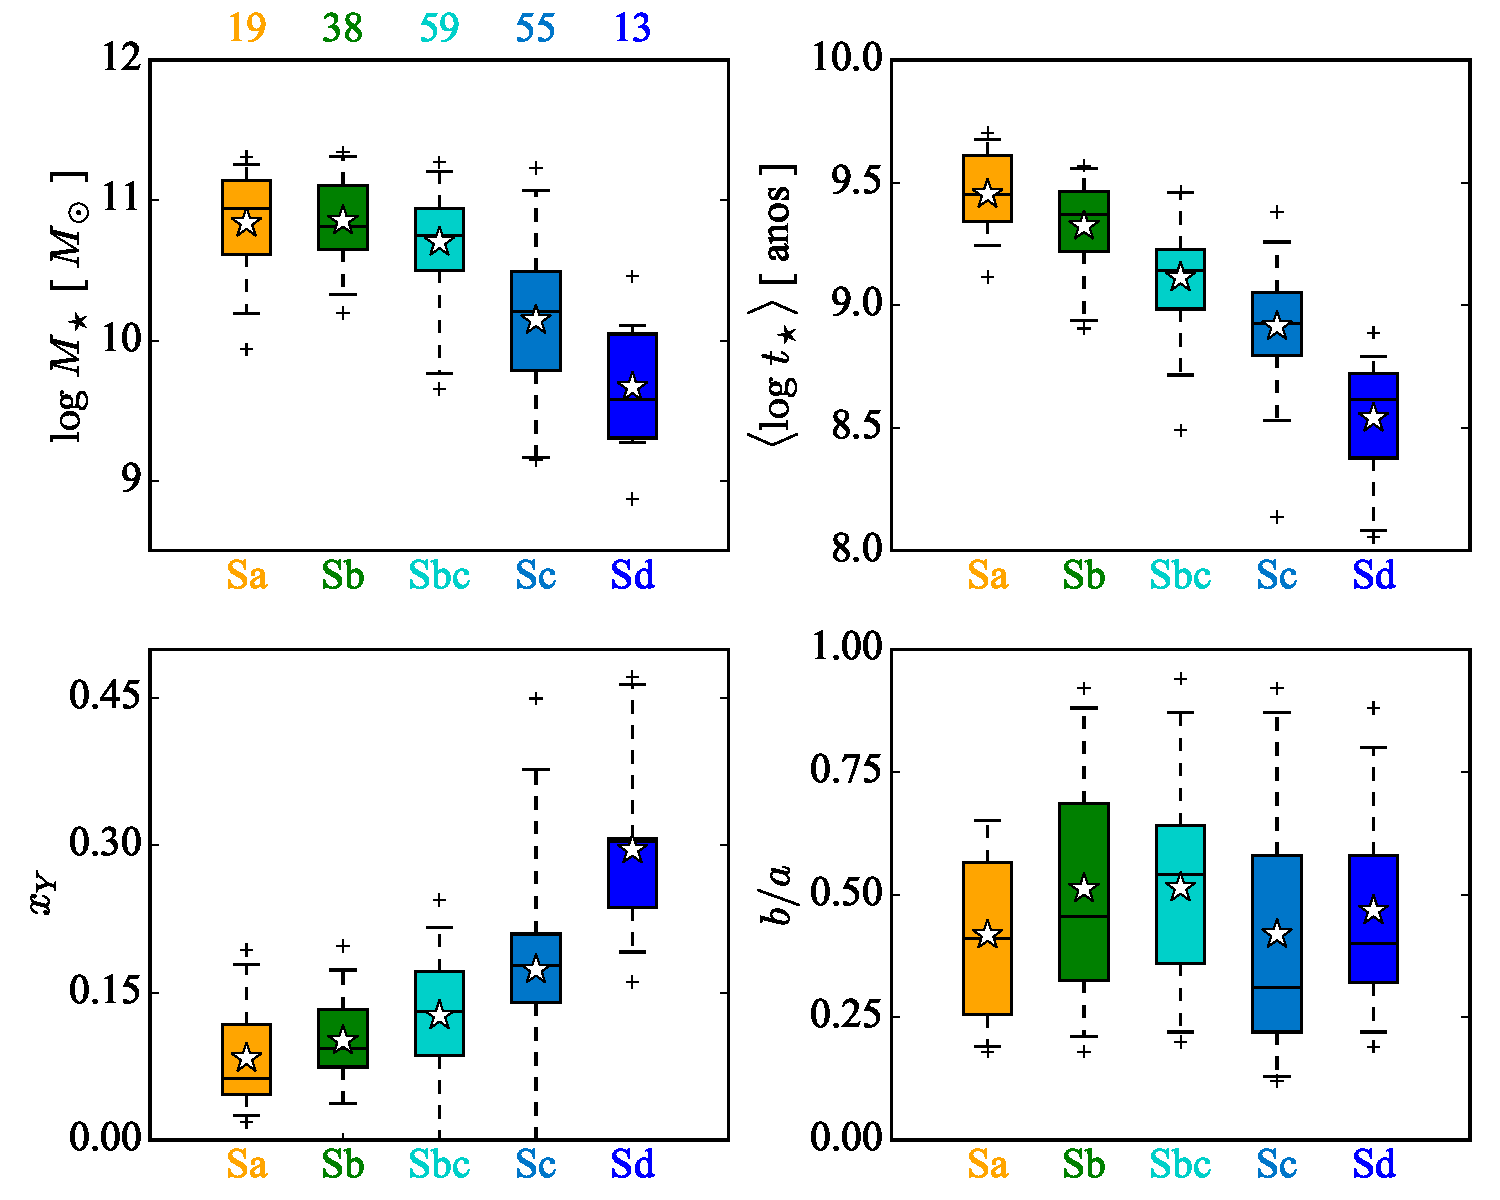
\includegraphics[width=0.99\textwidth]{figuras/sample_realsample_maskradius_integrated.pdf}
	\caption[Classificação por morfologia.]
	{Algumas propriedades separadas em classes morfológicas. Massa estelar ({\em painel a}), idade
estelar média ({\em painel b}), fração de luz proveniente das população jovens ({\em painel c}, $x_Y
\equiv x_Y(t_\star < 32 \times 10^6$ anos)$) e inclinação ({\em painel d}) de 305 galáxias espirais
da amostra observada do CALIFA. No primeiro painel, temos o número de galáxias dentro de cada classe
morfológica. Cada caixa tem altura definida pelo primeiro e terceiro quartil da distribuição dentro
de um tipo morfológico. Uma faixa preta marca a mediana e uma estrela a média. Em cada caixa, a
linha pontilhada vertical se estende mostrando o intervalo de $3\sigma$. Valores que ficam fora do
intervalo de $3\sigma$ são marcados por uma cruz vermelha.}
	\label{fig:amostraMorf}
\end{figure}

Estamos em fase de finalização de um artigo em que comparamos a relação entre a taxa de formação
estelar e a massa para diferentes classes morfológicas. Esse artigo já foi submetido e deve sair
logo agora no início de 2016.

\section{Perfis radiais}
\label{sec:amostra:rad}

Uma maneira interessante de analisar galáxias é produzir perfis radiais para as propriedades
físicas. Esse tipo de média azimutal (tanto em classes definidas por anéis circulares quanto em
anéis elípticos) diminui o espalhamento dos pontos. Para a análise individual de cada galáxia também
permite estudo da evolução das propriedades ao longo do raio. Quando colocamos todas as galáxias na
mesma análise, a vantagem dos {\em bins} radiais vem do balanceamento da influência de cada galáxia
quando analisamos todas juntas. Para que seja possível este ``empilhamento'' de galáxias, estas
médias radiais são feitas definindo-se um raio efetivo para cada galáxia. No nosso caso utilizamos
como raio efetivo aquele que comporta metade da luz da galáxia (HLR) e definimos 30 anéis com
espessura de 0.1 HLR (ou seja, indo até 3 HLR) partindo do pixel central de cada galáxia.

No artigo de \citet{GonzalezDelgado.etal.2014a} os autores discutem as estruturas radiais de algumas
propriedades estelares, aplicando este tipo de estudo para 107 galáxias no CALIFA. Nele são
derivados os raios de metade da luz (HLR) e de metade da massa ({\em half-mass radius} - HMR) e
deste resultado concluem que as galáxias são em geral 15\% mais compactas em massa do que em luz.
Também mostram que algumas propriedades, como idade estelar média, extinção por poeira e densidade
superficial de massa estelar são bem representados pelo seus valores medidas a 1 HLR.

Escolhemos utilizar perfis radiais em anéis elípticos neste trabalho, calculando a média entre todas
as zonas não mascaradas dentro de cana anel. Como um exemplo, podemos observar na Fig.
\ref{fig:K0140xYRadProf} três exemplos de mapas e perfis radiais ($x_Y$, $\tauVS$ e $\tauVN$) da
galáxia NGC1667 (objeto CALIFA 140). Em destaque (azul) temos o valor integrado para a galáxia.
Dentro de nosso trabalho utilizamos as medidas em zonas, em perfis radiais e quando necessário,
integradas (resolvendo para o disco ou para a galáxia completa), nos possibilitando portanto
verificar diferenças nestes tipos de abordagens.

\begin{figure}
	\centering
	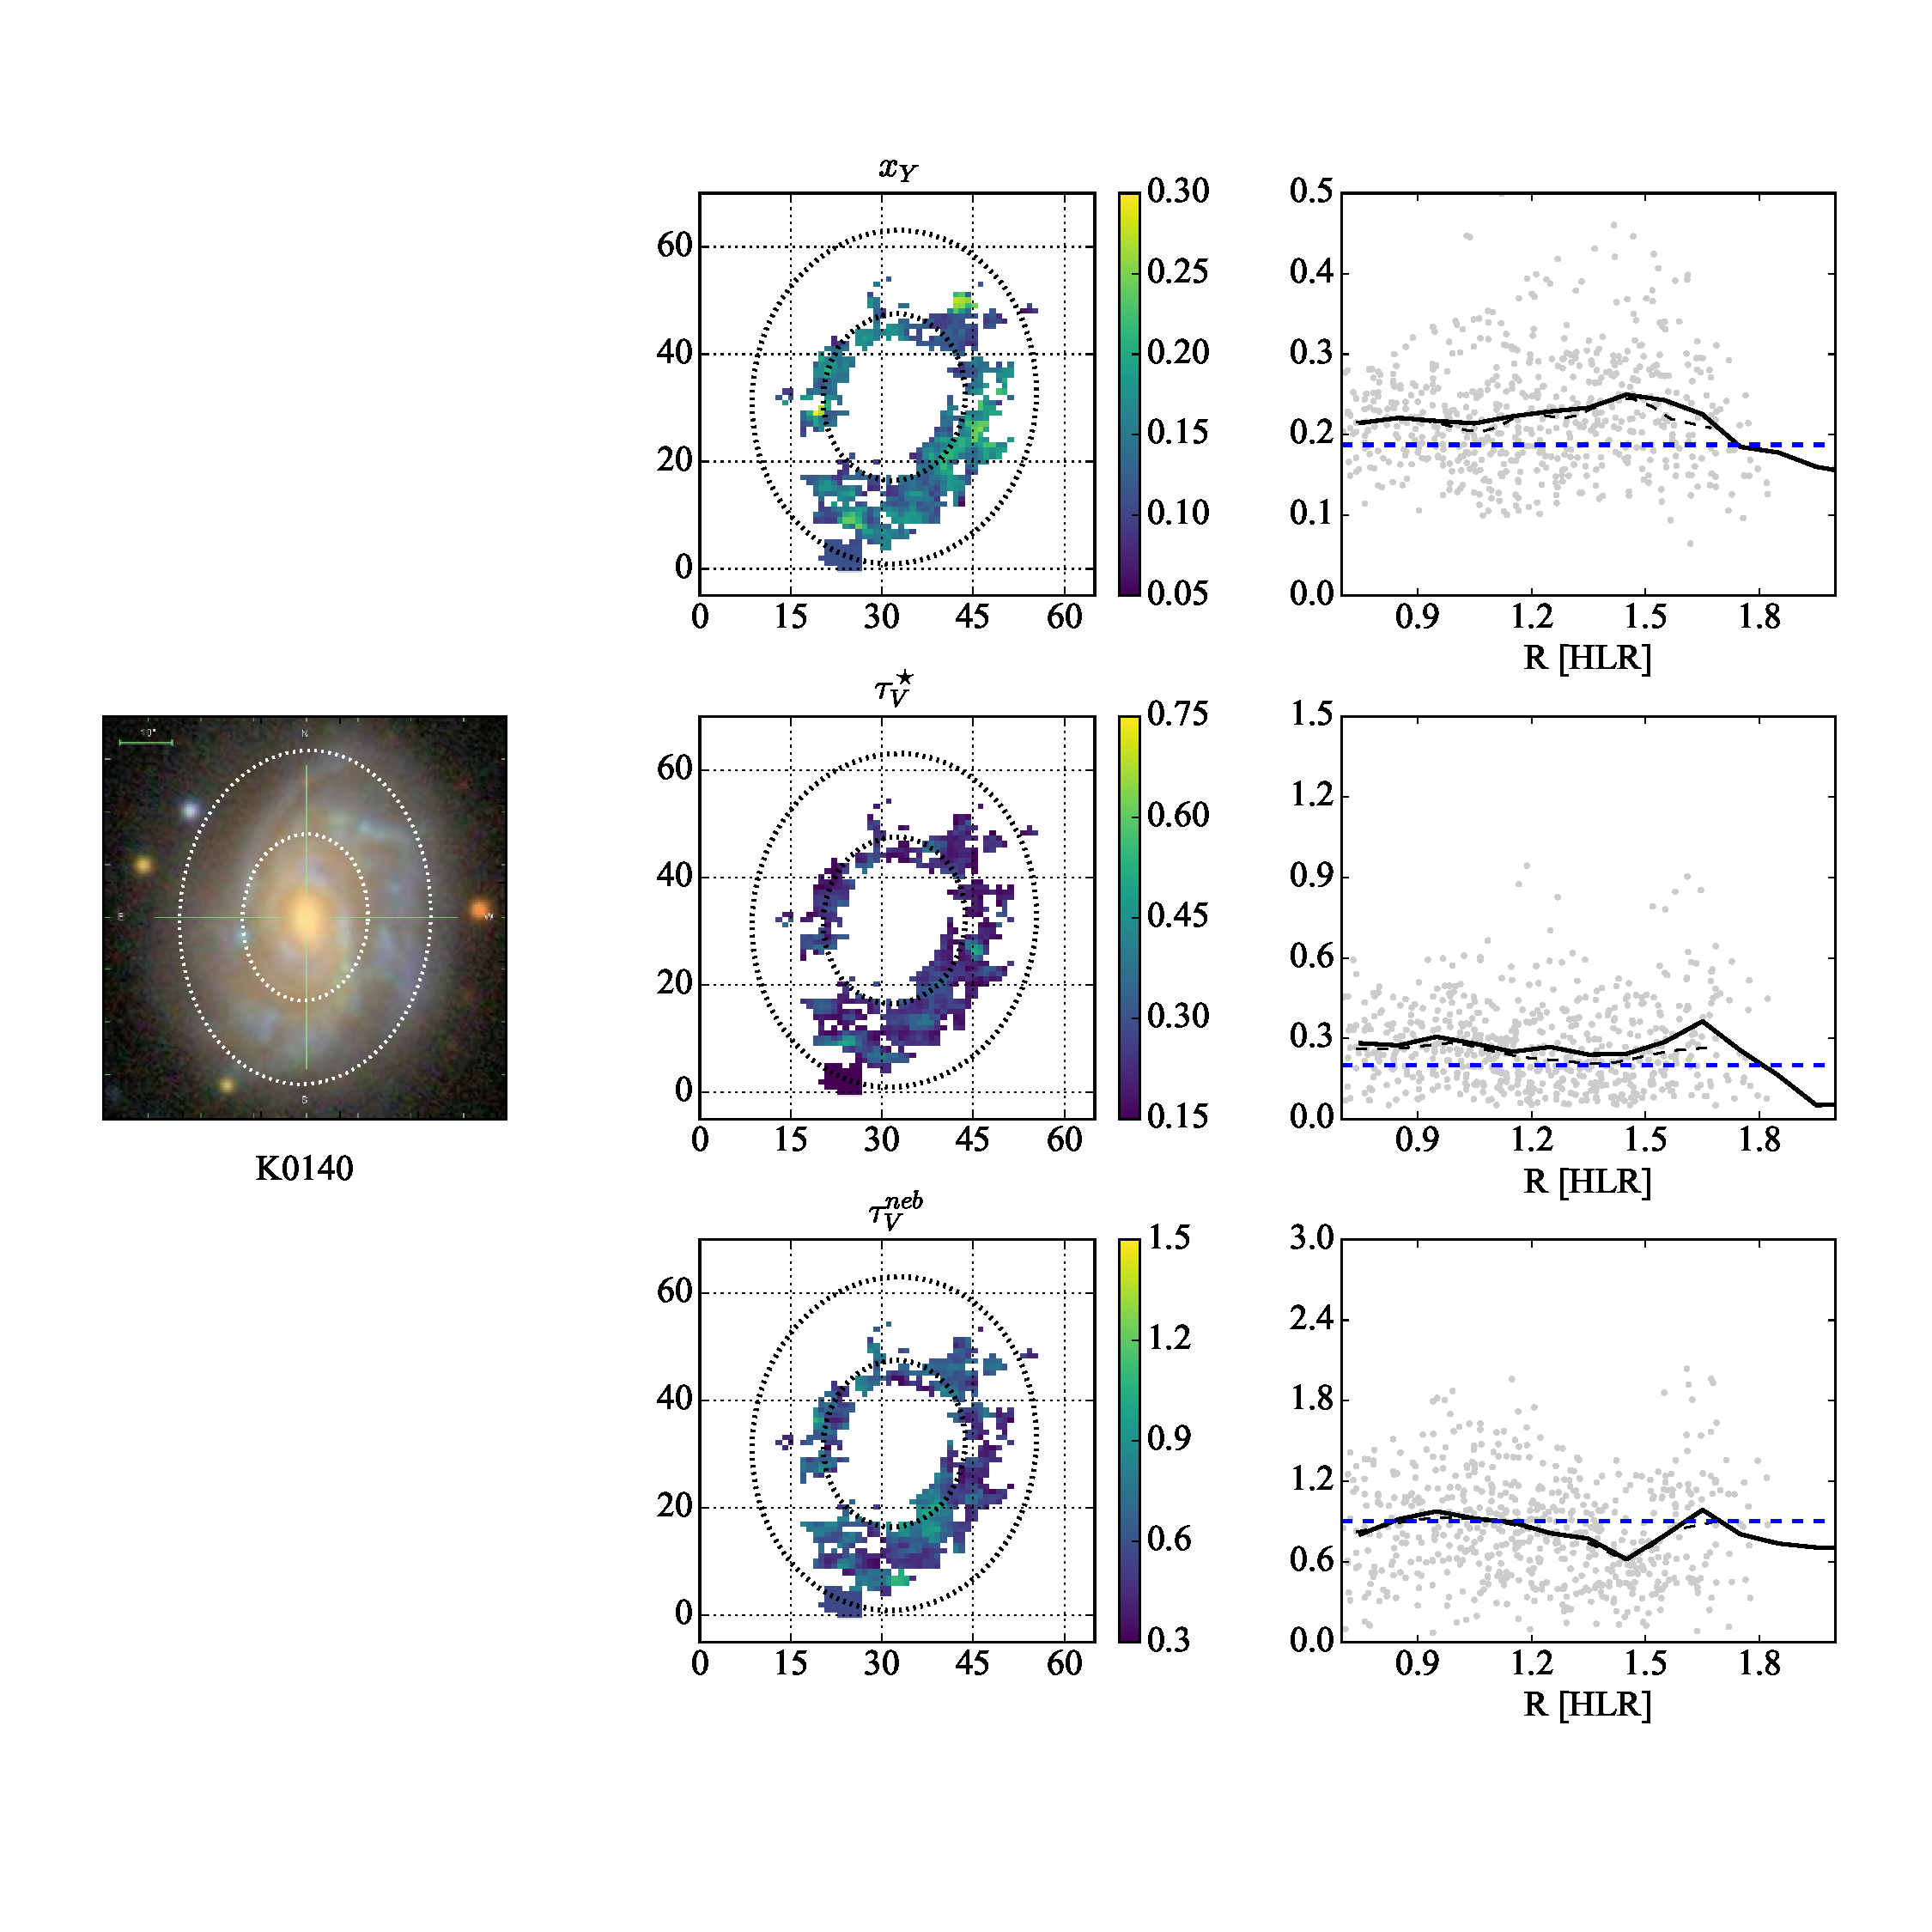
\includegraphics[width=0.99\textwidth]{figuras/K0140_xY_radialProfile_realsample.pdf}
	\caption[Imagem e exemplos de mapas e perfis radiais.]
	{Imagem do \SDSS da galáxia NGC1667 (CALIFA 140). Em cada fileira aparece o mapa e o perfil radial
da fração de luz proveniente das populações jovens ($x_Y$ - \emph{primeira fileira}), do
coeficiente de extinção resultante da síntese de populações estelares ($\tauVS$ - \emph{segunda
fileira}) e do coeficiente de extinção por decremento de Balmer ($\tauVN$ - \emph{terceira
fileira}). Nos mapas duas elipses concêntricas marcam 1 e 2 HLR. Em cada gráfico do perfil radial
aparece no fundo em cinza os valores para as zonas, em linha tracejada preta a mediana da
distribuição ao longo do raio e em azul tracejado o valor integrado para a galáxia, além do perfil
radial (linha preta contínua).}
	\label{fig:K0140xYRadProf}
\end{figure}

O perfil radial (entre 0.7 e 3 HLR) médio das principais propriedades utilizadas neste trabalho
podem ser vistas na Fig.\ \ref{fig:RadProfProps} juntamente com seus histogramas na Fig.
\ref{fig:HistoRadProfProps}. Elas são muito importantes em todos os aspectos que abordaremos:
formação estelar, poeira e a conversão de densidade superficial de poeira em densidade superficial
de gás em discos de galáxias espirais. Podemos ver que existem alguns gradientes negativos (crescem
de fora para dentro) bem definidos de densidade superficial da taxa de formação estelar
($\Sigma_{\mathrm{SFR}}$), a metalicidade nebular, ($\log O/H$), densidade superficial de massa
estelar ($\mu_\star$). Outras propriedades parecem não variar muito dentro do disco. Alguns perfis
mudam de tendência ao passar de 2 HLR, mas vale ressaltar que na maioria das distribuições, os
pontos acima de 2 HLR ultrapassam $1\sigma$ da distribuição. Embora não seja tão forte, existe um
gradiente positivo na fração em luz de populações jovens.

\begin{figure}
	\centering
	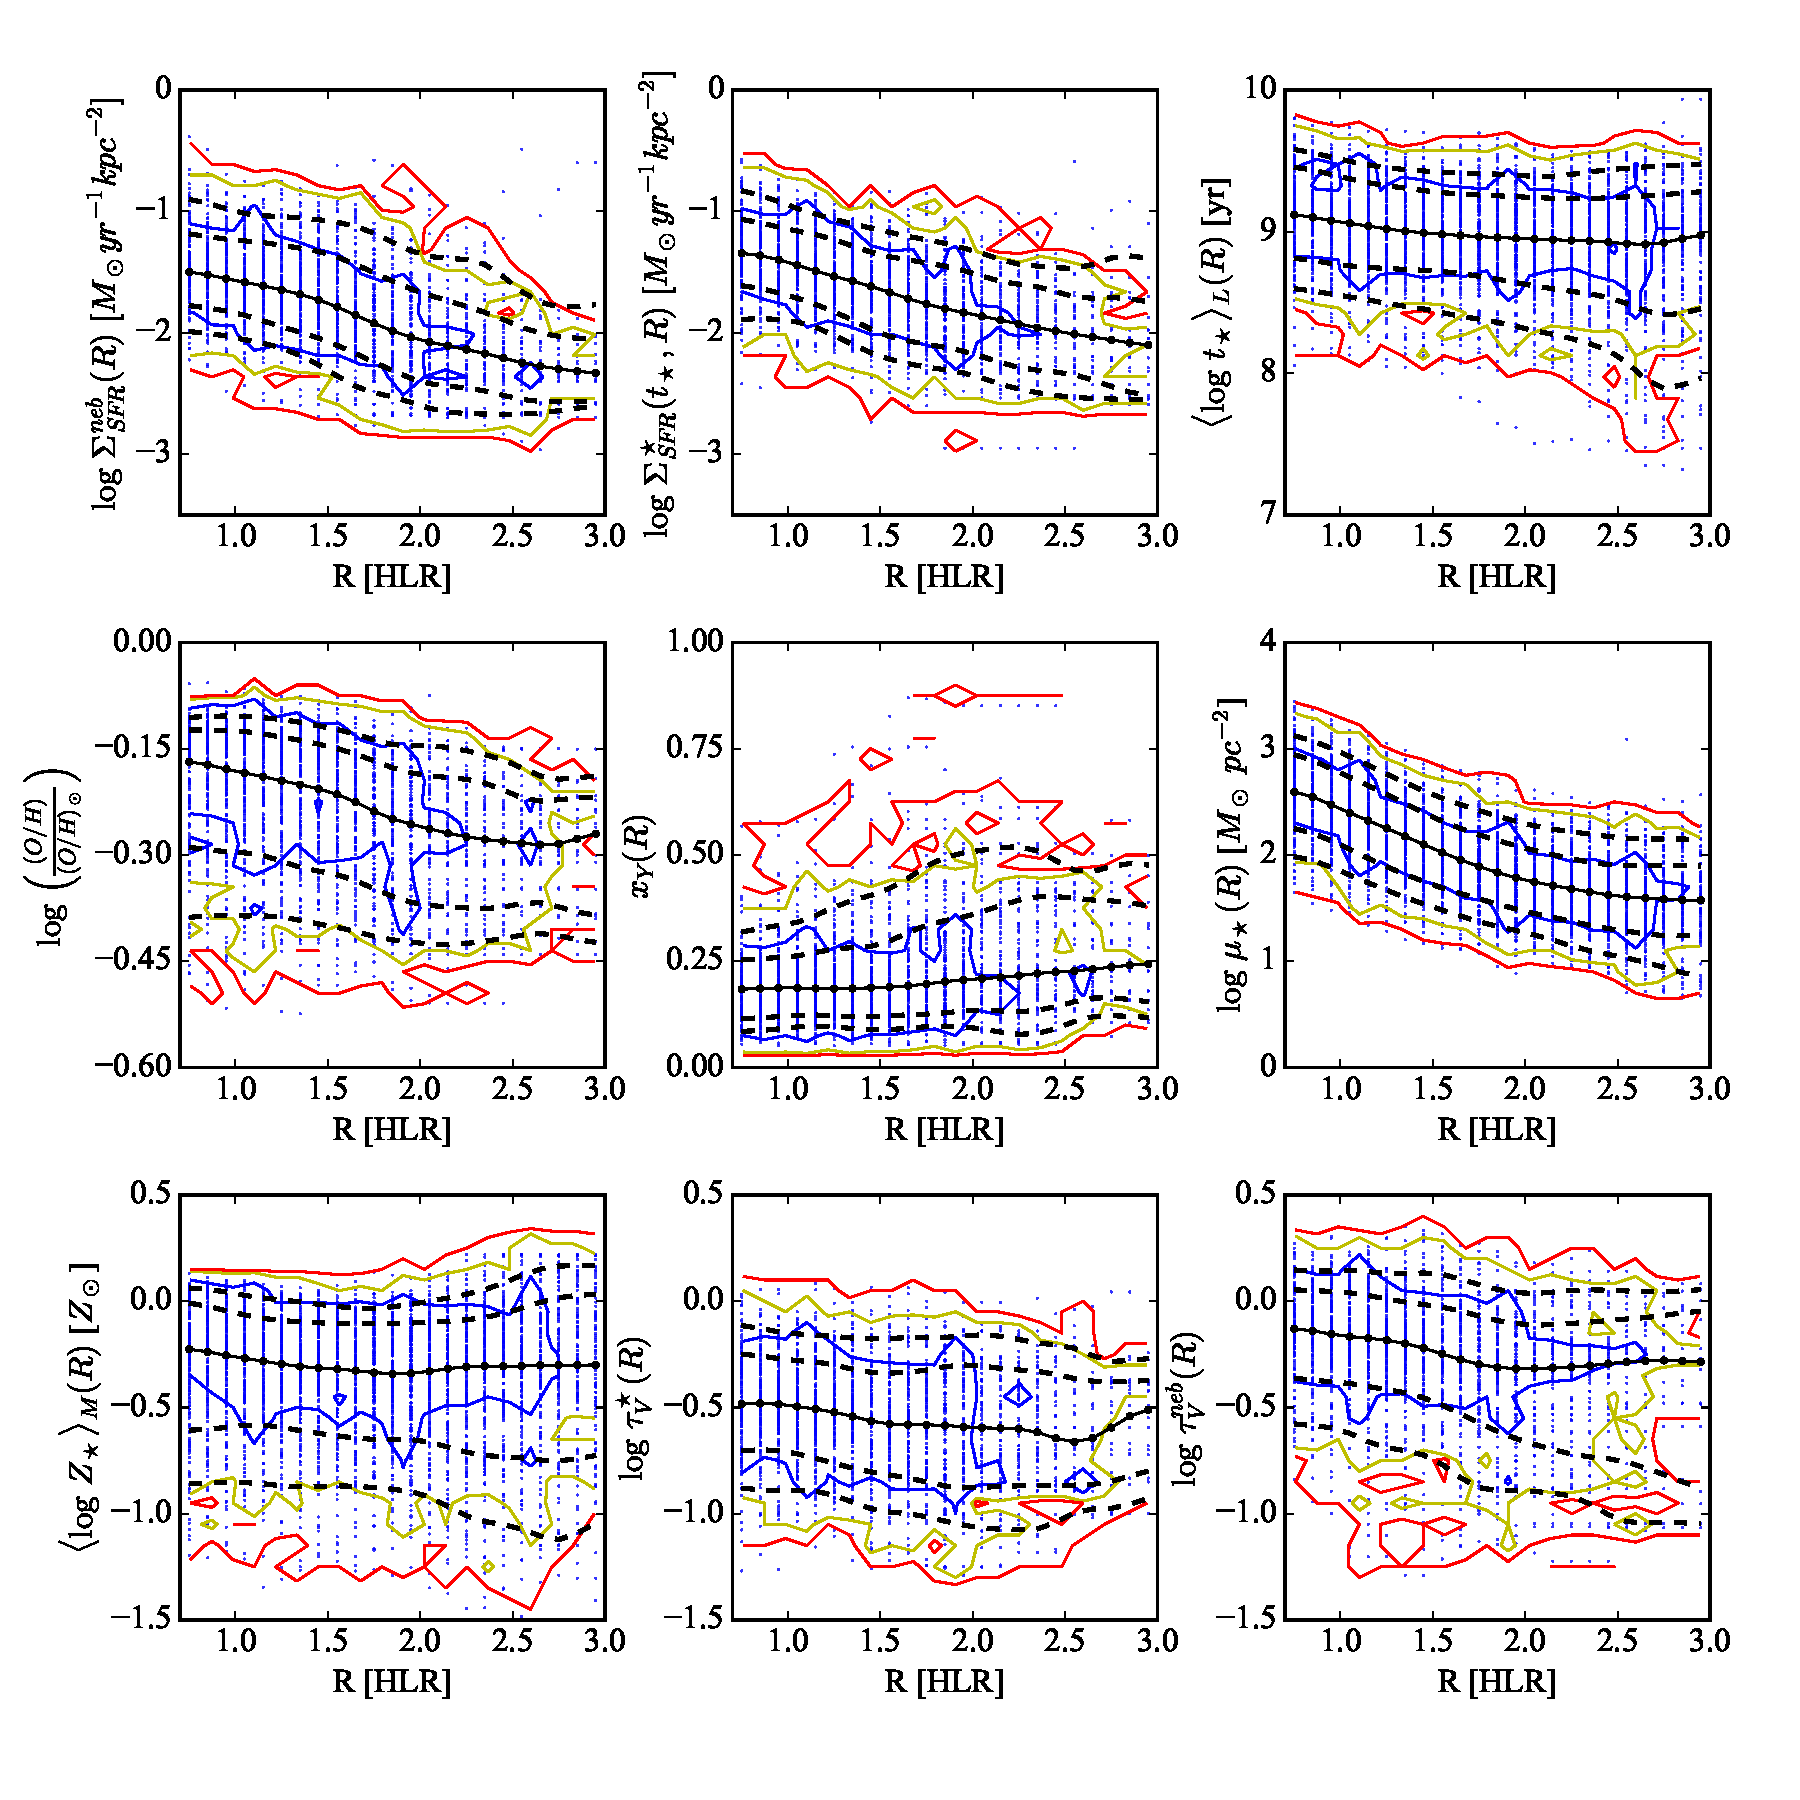
\includegraphics[width=0.9\textwidth]{figuras/props_R.pdf}
	\caption[Perfis radiais das propriedades físicas.]
	{Perfis radiais médios (entre 0.7 e 3 HLR) das principais propriedades físicas abordadas neste
trabalho. Densidade superficial da taxa de formação estelar detectada por \Halpha e pela síntese
({\em painéis a e b}), idade média das populações estelares ({\em painel c}), metalicidade nebular
({\em painel d}), fração em luz de populações jovens ({\em painel e}), densidade superficial de
massa estelar ({\em painel f}), metalicidade média das populações estelares ({\em painel g}),
coeficiente de extinção da síntese e do decremento de Balmer ({\em painéis h e i}). Em cada painel
vemos também os contornos definindo $1\sigma$, $2\sigma$ e $3\sigma$ da distribuição. As linhas
marcam a mediana (linha contínua) e os 5, 16, 64, 95 percentis (linhas tracejadas).}
	\label{fig:RadProfProps}
\end{figure}

\begin{figure}
	\centering
	\includegraphics[width=0.99\textwidth]{figuras/histo_props_R.pdf}
	\caption[Histogramas dos perfis radiais das propriedades físicas.]
	{Histogramas normalizados de todas as propriedades físicas da Fig.\ \ref{fig:RadProfProps}. Os
valores no canto superior direito marcam a média, mediana, desvio padrão, máximo e mínimo das
distribuições.}
	\label{fig:HistoRadProfProps}
\end{figure}

% Figuras:
% - histograma tipos - histograma massa - influências dos cortes em tauV, raio e x_Y - Anexo: Lista
% de galáxias com massa, redshift, idade, etc ...
%% End of this chapter
